\newpage
\appendix

\section{KUKA youBot Design Specification}\label{app:kinematics}

\begin{figure}[h]
  \centering
  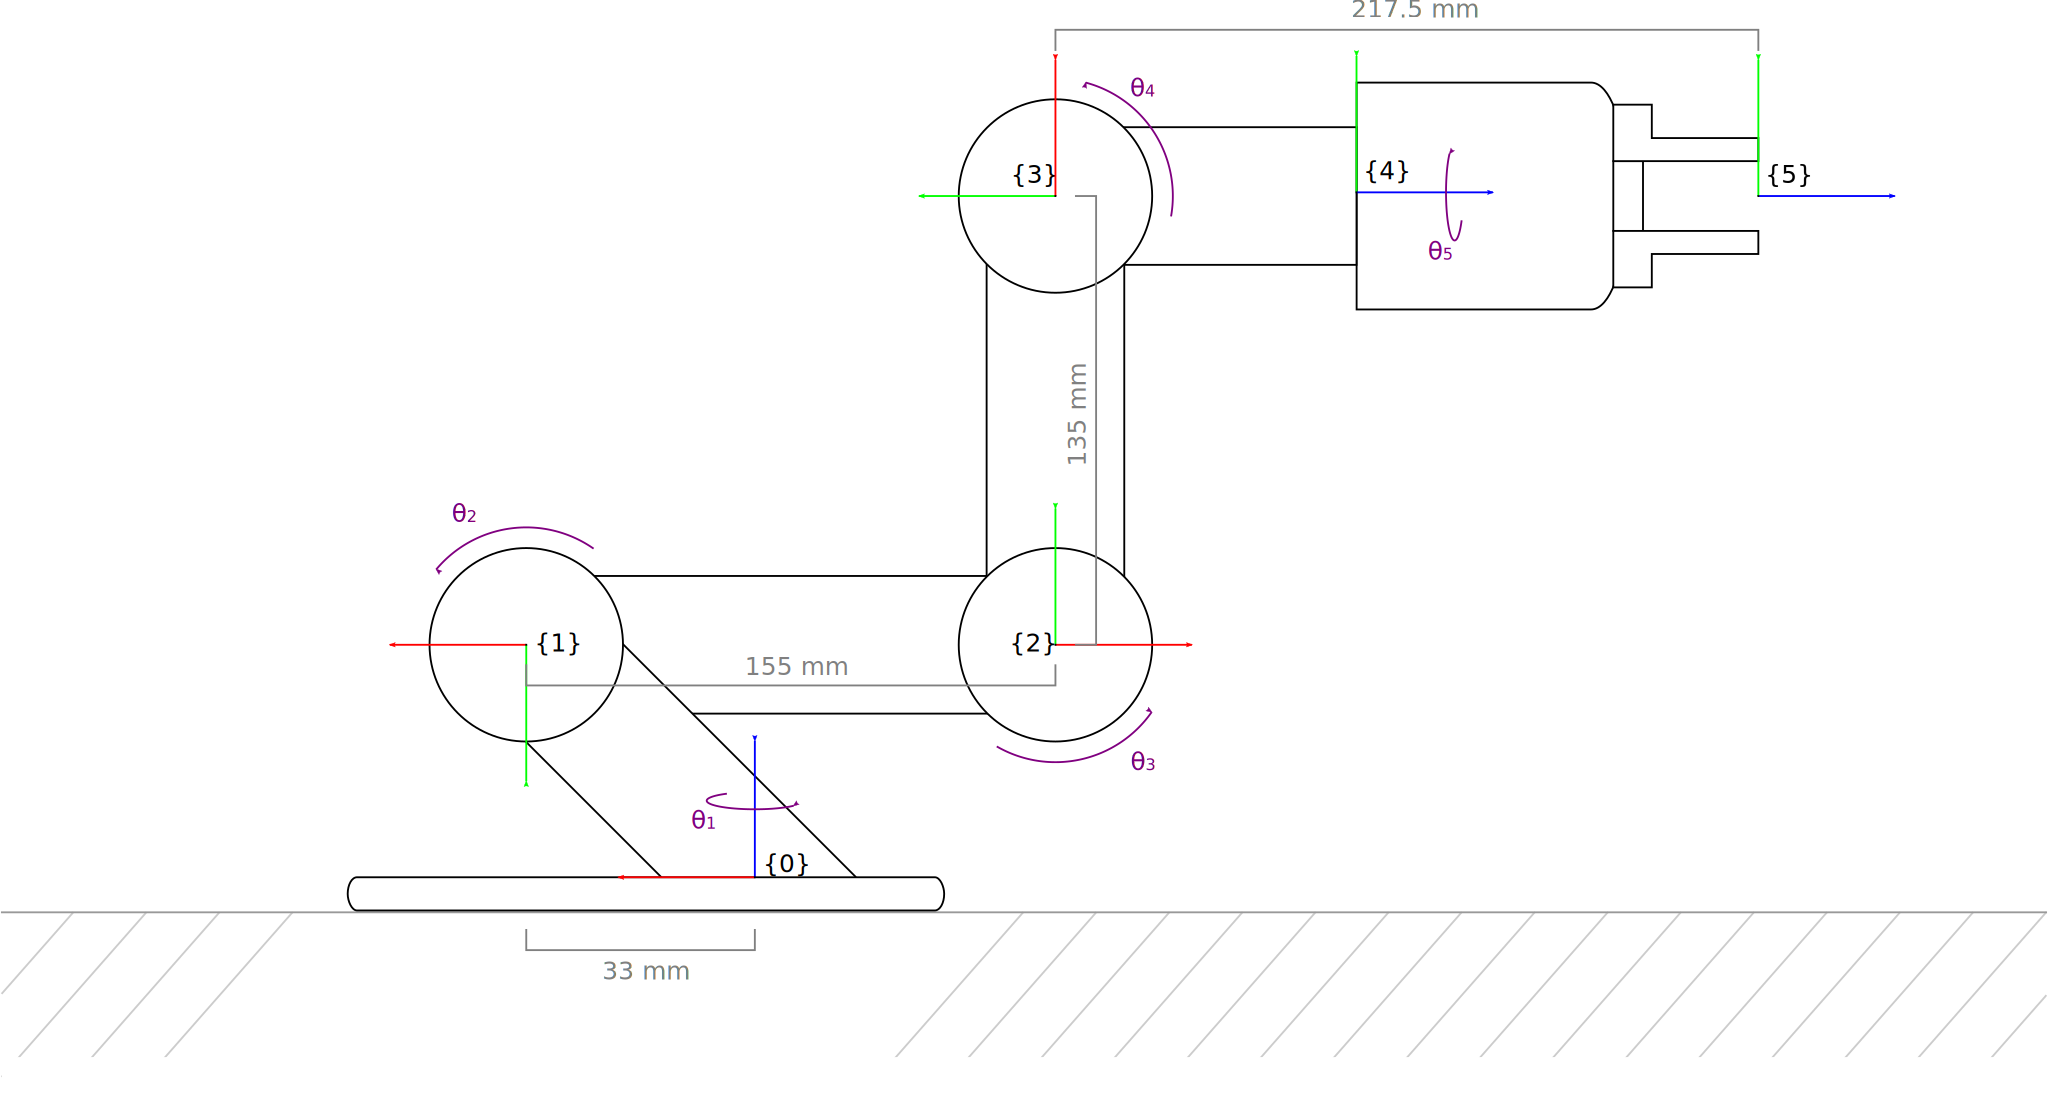
\includegraphics[width=\textwidth]{figures/p2/youBot_specs.pdf}
  \caption{Informal design specification for the KUKA youBot manipulator arm, which has five
    revolute joints and a two-finger gripper. The angle of joint $i$ is given by $\theta_i$, and the
    direction in which the angle is measured is shown with a purple arrow. Each link in the arm has a
    frame rigidly attached to it, and the $x$-, $y$-, and $z$-axes of the frame are shown in red, green,
    and blue, respectively (the one unshown axis for each frame points either out of or into the page).
    Note that $z_i$ is the axis of rotation for joint $i + 1$, \textbf{not} joint $i$. The frames are
    attached in this manner so that when joint $i$ is actuated, link $i$ and its attached frame $\{i\}$
    move. Finally, note that since axes $z_3$ and $z_4$ intersect, the origin of frame $\{4\}$ can be
    placed at any point along $z_4$. We have depicted it at the wrist for the sake of the visual, but in
  practice we would place it at the intersection of $z_3$ and $z_4$ to simplify the math.}
\end{figure}

\newpage

\section{NumPy Overview}\label{app:numpy}

\begin{description}
  \item[Importing NumPy] First, make sure to import NumPy: \texttt{import numpy as np}
  \item[Constructing an array] A NumPy array can be any number of dimensions. To create a
    $n$-dimensional array, you can use \texttt{np.array()}. For example, \texttt{a\_1D =
      np.array([1.,2.,3.])} creates a 1D array of floats, and \texttt{a\_2D =
    np.array([[2,2],[0,1]])} creates a 2D array of ints where the first row is [2, 2] and the second
    row is [0, 1].
  \item[Special arrays] NumPy includes some useful functions to create special arrays. One such
    function is \texttt{np.zeros(shape)}, which returns a $n$-dimensional array of the specified
    shape (a tuple specifying each of the $n$ dimensions). For instance, \texttt{np.zeros((3,2))}
    returns a $3 \times 2$ array of 0s. Another useful function is \texttt{np.identity(n)}, which
    returns a $n \times n$ identity matrix.
  \item[Constructing a matrix] A NumPy matrix is just a special 2D NumPy array. Use
    \texttt{np.matrix()} to create a matrix. For example, \texttt{m = np.matrix([[2,2],[0,1]])}
    creates a matrix with the same values as \texttt{a\_2D} from above. However, while they may be
    very similar and you can do the same things with both, the matrix and array types are not
    exactly the same. Besides the fact that a matrix can only be 2D, an important difference is in
    matrix multiplication, as described next.
  \item[Matrix multiplication] To perform matrix multiplication with the matrix type, you can simply
    use the * operator. For example, we can multiply the matrix \texttt{m} we defined above by doing
    \texttt{m}*\texttt{m}. If you're working with 2D matrices, the matrix type is convenient since
    matrix multiplication is very intuitive. \textbf{Be careful:} In this case, the * operator
    performs matrix multiplication like you might expect. However, if you use $n$-dimensional arrays
    instead of matrices, the * operator will multiply the arrays element-wise. You can do normal
    matrix multiplication with arrays by using NumPy's \texttt{dot()} function. For example,
    \texttt{a\_2D.dot(a\_2D)}, or alternatively \texttt{np.dot(a\_2D,a\_2D)}, will return the same
    matrix product as \texttt{m}*\texttt{m}, and these are NOT equal to
    \texttt{a\_2D}*\texttt{a\_2D}.
  \item[Inverse and transpose] Getting the transpose of a matrix/array with NumPy is easy. You just
    need to use \texttt{.T} (e.g. \texttt{m.T} or \texttt{a\_2D.T}). You can get the inverse of a
    square matrix/2D array using \texttt{np.linalg.inv()}. For example: \texttt{np.linalg.inv(m)}.
  \item[Indexing] You can access specific parts of an array/matrix by indexing particular cells like
    you would expect (e.g. \texttt{m[1,0]} would return 0). You can also use slicing to get subsets
    of a matrix/array. For example, \texttt{m[:,1]} returns the second column of \texttt{m}, where
    the colon selects all of the rows and the 1 specifies the column we want.
\end{description}

For a more in-depth NumPy guide, you can read the quickstart tutorial
\href{https://docs.scipy.org/doc/numpy-dev/user/quickstart.html}{here}.
